% File: basic_elements.tex
\documentclass{standalone}
\usepackage{pgfplots}
\pgfplotsset{compat=1.18}
\usepackage[american]{circuitikz}
\usepackage{cmbright}

\definecolor{myred}{RGB}{170,0,0}
\definecolor{myblue}{RGB}{0,0,220}

\ctikzset{bipoles/resistor/height=0.2}
\ctikzset{bipoles/resistor/width=0.5}

\begin{document}
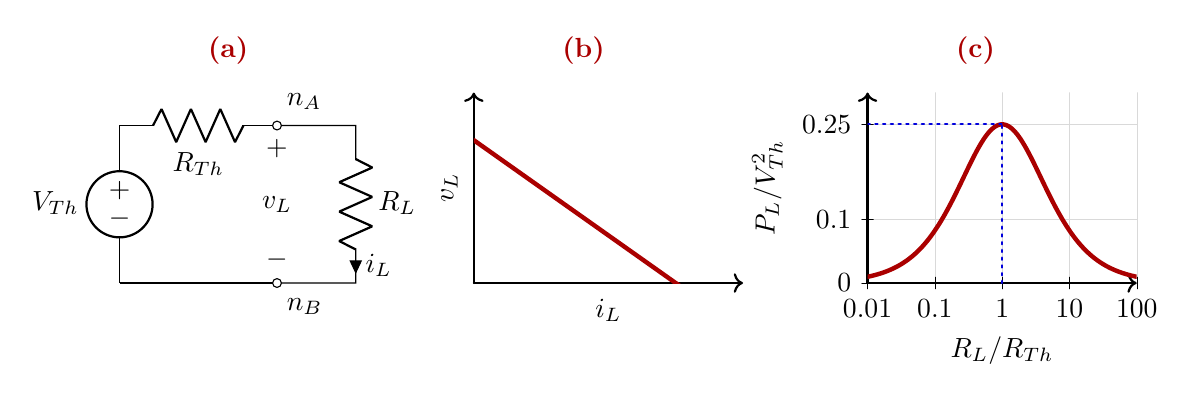
\begin{tikzpicture}
    % Subtitle for the circuit.
    \node[anchor=north west, color=myred] at (1.0, 3.25) {\textbf{(a)}};
    % --- Circuit (top left)
    \begin{scope}
        % Nodes A and B
        \draw (2, 2) node[ocirc] (A) {};
        \draw (A) node[right, yshift=3mm] {$n_A$};
        \draw (2, 0) node[ocirc] (B) {};
        \draw (B) node[right, yshift=-3mm] {$n_B$};

        % Voltage source and lower wire
        \draw (0, 0) to[V, l={$V_{Th}$}, invert] (0, 2) to[R, l_=$R_{Th}$] (A);
        \draw (0, 0) -- (B);

        % Resistor and upper wire
        \draw (A) to ++(1, 0)
            to[R, l=$R_L$, i^>=$i_L$] ++(0, -2)
            to (B);

        % Voltage label across A and B
        \draw (A) to[open, v^=$v_{L}$] (B);
    \end{scope}

    % Plot of v_L vs i_L (top right)
    \begin{scope}[xshift=4.5cm]
        % Subtitle for the circuit.
        \node[anchor=north west, color=myred] at (1.0, 3.25) {\textbf{(b)}};
        \begin{axis}[
            width=5cm,
            height=4cm,
            xlabel={$i_L$},
            ylabel={$v_L$},
            xmin=0, xmax=4,
            ymin=0, ymax=2,
            samples=100,
            domain=0:4,
            thick,
            axis lines=left,
            axis line style={->},
            xtick=\empty,
            ytick=\empty,
            % tick style={black},
            % grid=both,
            % major grid style={line width=.2pt,draw=gray!30},
            % minor grid style={line width=.1pt,draw=gray!10},
            line cap=round
        ]
        \addplot[myred, ultra thick] {1.5 - x*0.5}; % Linear drop: Vth - i*Rth
        \end{axis}
    \end{scope}

    % Plot of of the power transfer (bottom left)
    % Plot of the power transfer (bottom right)
    \begin{scope}[xshift=9.5cm]
        % Subtitle for the circuit.
        \node[anchor=north west, color=myred] at (1.0, 3.25) {\textbf{(c)}};
        \begin{axis}[
            width=5cm,
            height=4cm,
            xlabel={$R_L / R_{Th}$},
            ylabel={$P_L / V_{Th}^2$},
            xmode=log,
            log basis x=10,
            xtick={0.01, 0.1, 1, 10, 100},
            xticklabels={$0.01$, $0.1$, $1$, $10$, $100$},
            ytick={0,0.1,0.25,0.5,0.75,1},
            ymin=0, ymax=0.3,
            domain=0.01:100,
            samples=200,
            thick,
            grid=both,
            axis lines=left,
            major grid style={line width=.2pt,draw=gray!30},
            minor grid style={line width=.1pt,draw=gray!10},
            axis line style={->},
            tick style={black},
            line cap=round
        ]
        \addplot[myred, ultra thick] {x / (x + 1)^2};
        % \node[myblue] at (axis cs:1,0.25) {max};
        \draw[dotted, myblue] (axis cs:1,0) -- (axis cs:1,0.25);
        \draw[dotted, myblue] (axis cs:0.01,0.25) -- (axis cs:1,0.25);
        \end{axis}
    \end{scope}
\end{tikzpicture}
\end{document}